\documentclass[conference]{IEEEtran}
\IEEEoverridecommandlockouts
% The preceding line is only needed to identify funding in the first footnote. If that is unneeded, please comment it out.
\usepackage{biblatex}
\usepackage{amsmath,amssymb,amsfonts}
\usepackage{algorithmic}
\usepackage{graphicx}
\usepackage{textcomp}
\usepackage{xcolor}
\def\BibTeX{{\rm B\kern-.05em{\sc i\kern-.025em b}\kern-.08em
    T\kern-.1667em\lower.7ex\hbox{E}\kern-.125emX}}

\addbibresource{citations.bib}

\begin{document}

\title{Graph Databases for Use with Timeseries IoT Datasets}

\author{\IEEEauthorblockN{Colter Snyder}
\IEEEauthorblockA{\textit{Department of Computer Science} \\
\textit{Colorado School of Mines}\\
Golden, Colorado, USA \\
csnyder1@mines.edu}
}

\maketitle

\begin{abstract}
The wide spread proliferation of Internet of Things (IoT) devices
have brought up many questions and concerns about their security
and what they do with data. Many solutions have appeared using 
various solutions such as IoT Inspector \cite{IoTInspector}. 
However, these solutions don't make use of the unique capabilities
and efficiencies that graph databases provide. This paper seeks
to use a graph database in order to answer challenging questions 
about IoT devices particularly within the realm of timeseries datasets.
\end{abstract}

\begin{IEEEkeywords}
IoT, graphical databases, databases, systems
\end{IEEEkeywords}

\section{Introduction}
Smart homes are everywhere now adays, from lights to door locks, TVs to speakers.
It seems that these devices, which are refered to by their collective as Internet of Things or IoT devices, are in every home.
With all these new devices come a whole slew of concerns about privacy and security \cite{IoTInspector}.
There are many papers that explore these concerns, what this paper seeks to persue is how to efficiently analyze
data collected from these devices such that people may infer various aspects about their devices. In particular,
this paper seeks to see what what info can be garnered from timeseries datasets. Such aspects could include
anything from what the device is doing to answering if a device is attacking the network and how.

It was decided that using a graph database could provide answers to these questions
more efficiently and easily than a relational database. The primary advantage for use in this paper
is the fact that graph databases are great for use with densely connected data \cite{GraphSurvey}.
On top of this, they are very quick to query and will give a result relatively quickly compared to
other solutions \cite{GraphSurvey}.


\section{Related Works}
There are many current systems that implement different components of the general idea of graphical databases for
IoT device management andanomoly detection, but none put these components together. \textit{IoT Inspector} is a great
tool that performs the task of monitoring using a form of a relational database, but not a graphical one \cite{IoTInspector}.
The authors of \textit{The Graph of Things} created such a system for aggregating IoT devices worldwide \cite{GraphofThings}; 
However, these systems are not built for small networks or home users.

\section{Methodology}
The first step in this project was choosing the technology that was to be used. It was decided to use Neo4J
and Python for the tech stack. 

\section{Results}

\begin{figure}[h]
    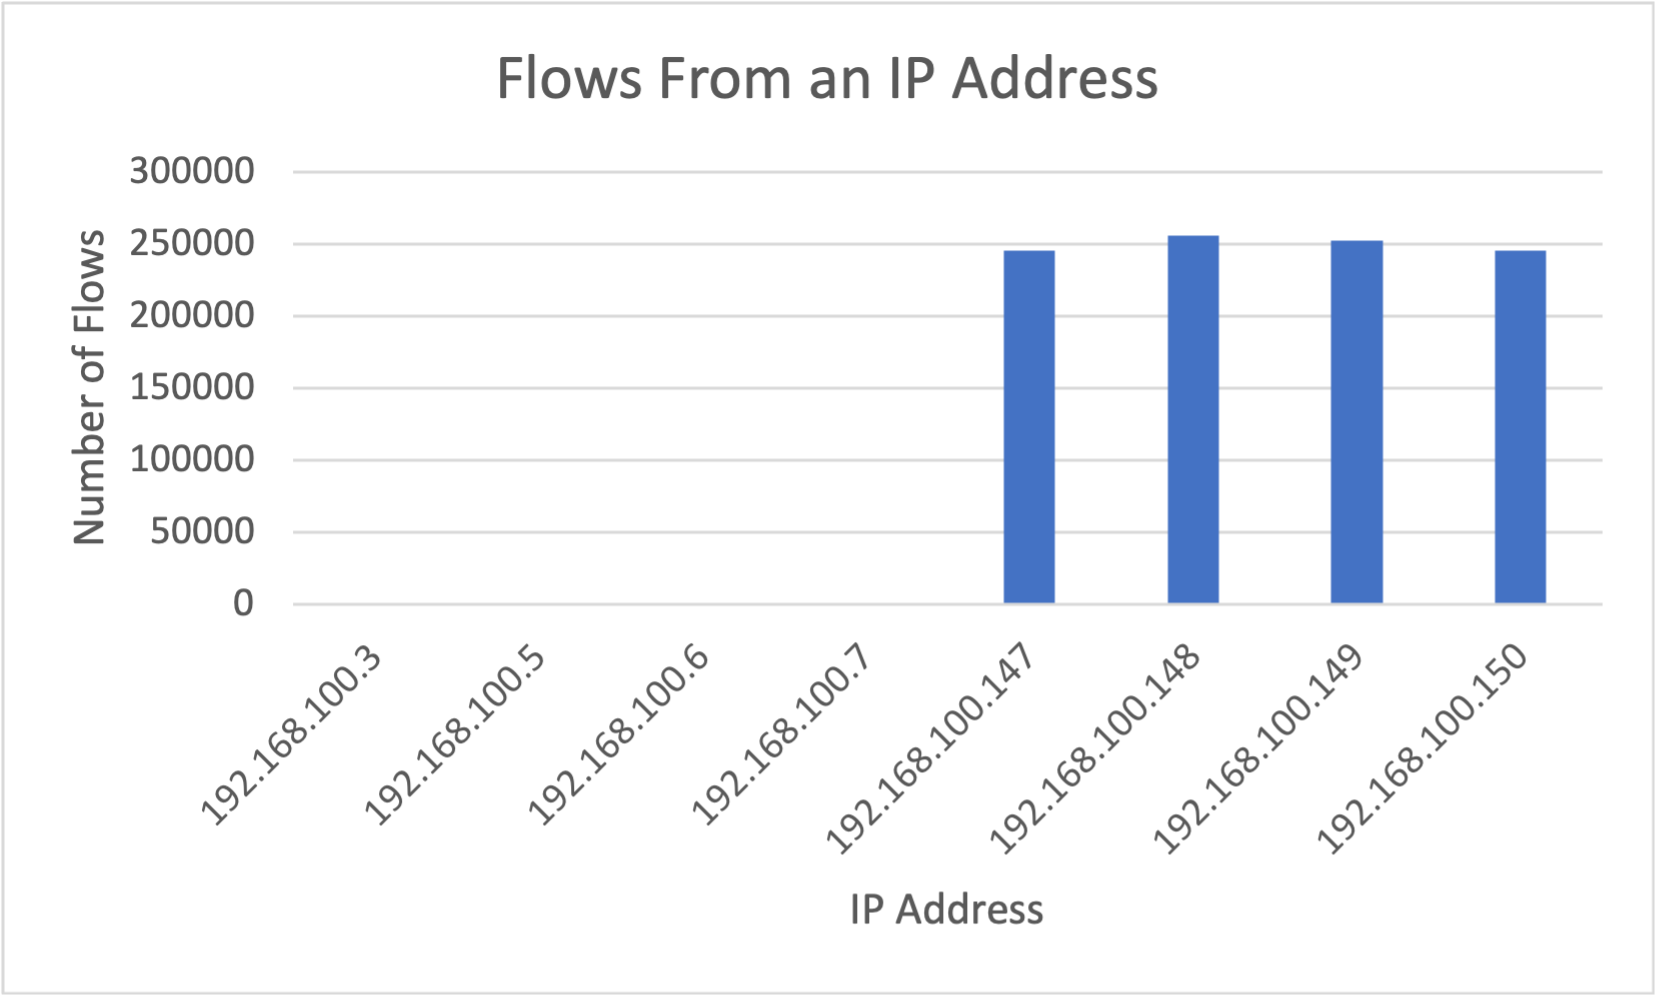
\includegraphics[width=8cm]{Figure1.png}
    \centering
    \caption{The number of flows that were sent from particular IP addresses}
    \label{fig:flowfrom}
\end{figure}

\begin{figure}[h]
    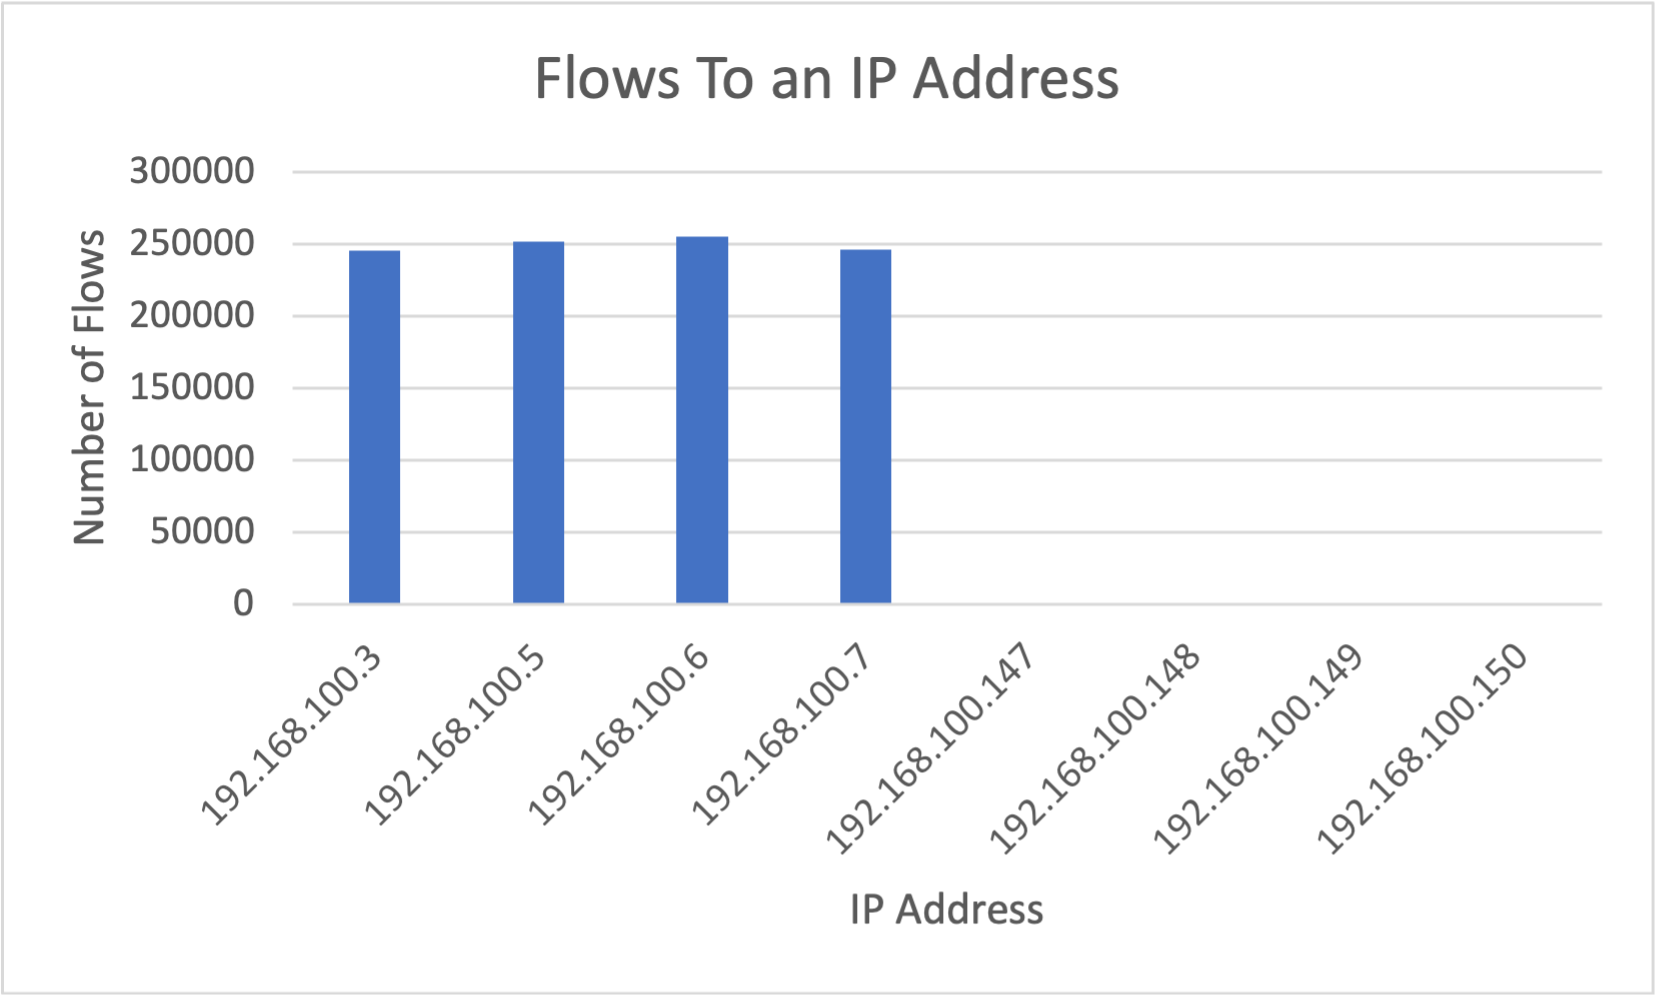
\includegraphics[width=8cm]{Figure2.png}
    \centering
    \caption{The number of flows that were sent to particular IP addresses}
    \label{fig:flowto}
\end{figure}

\begin{figure}[h]
    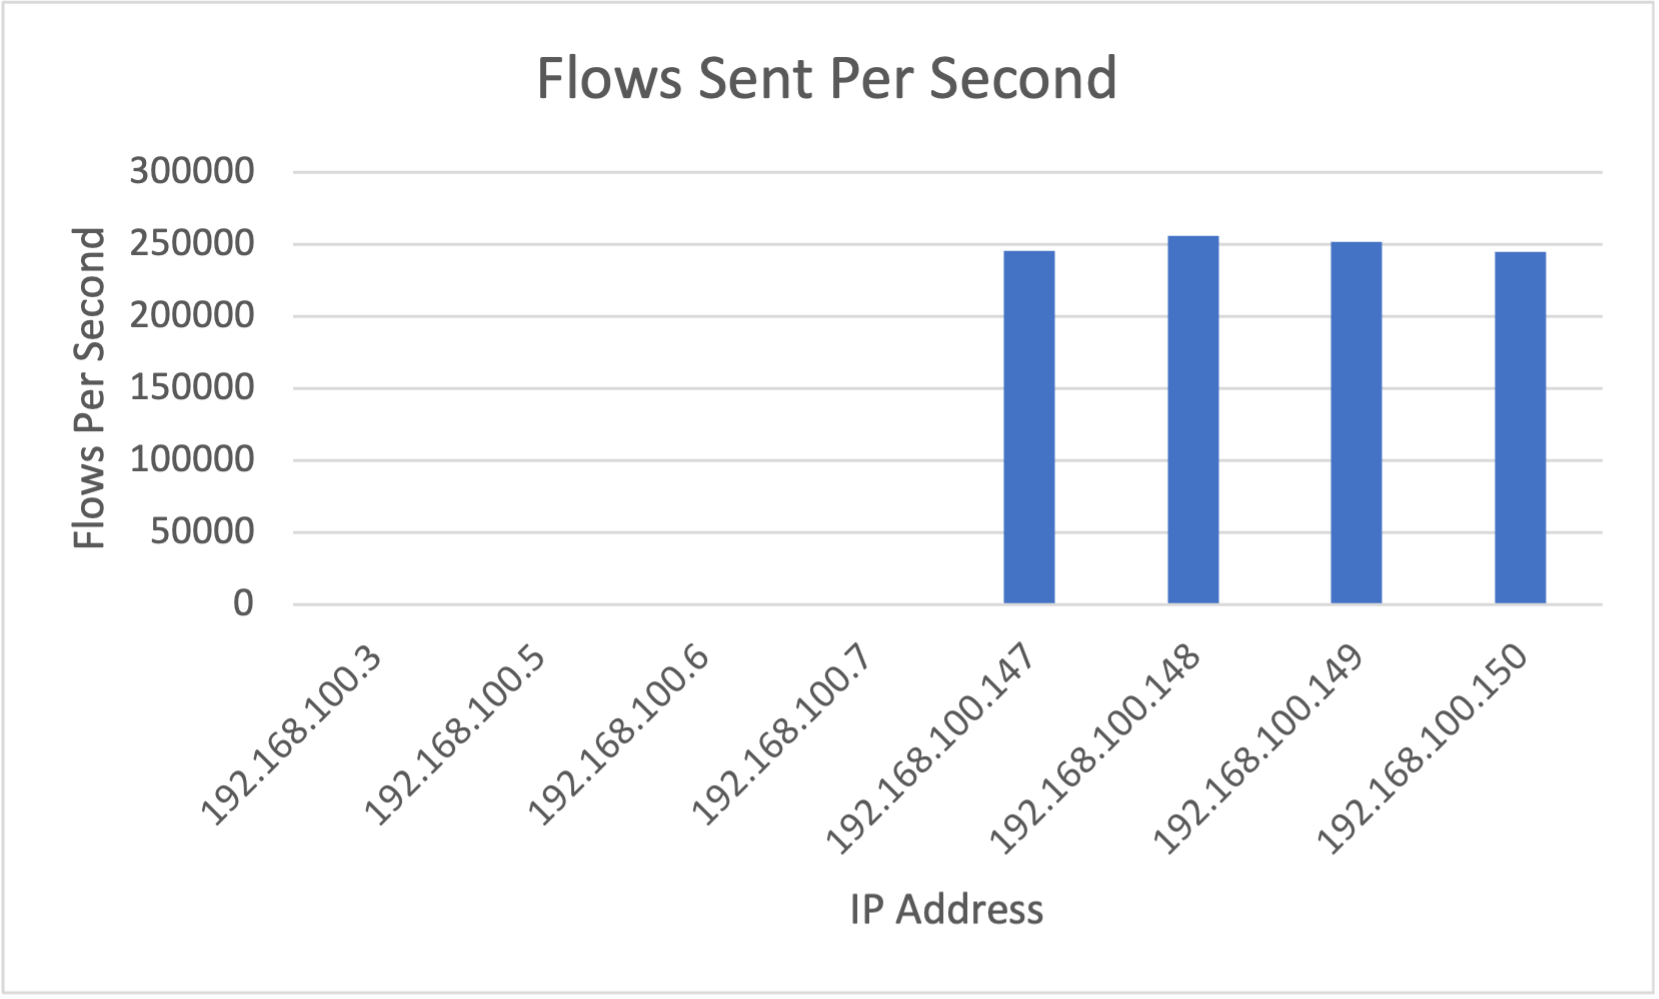
\includegraphics[width=8cm]{Figure3.png}
    \centering
    \caption{The number of flows that were sent from particular IP addresses per second}
    \label{fig:sentfrompersec}
\end{figure}

\begin{figure}[h]
    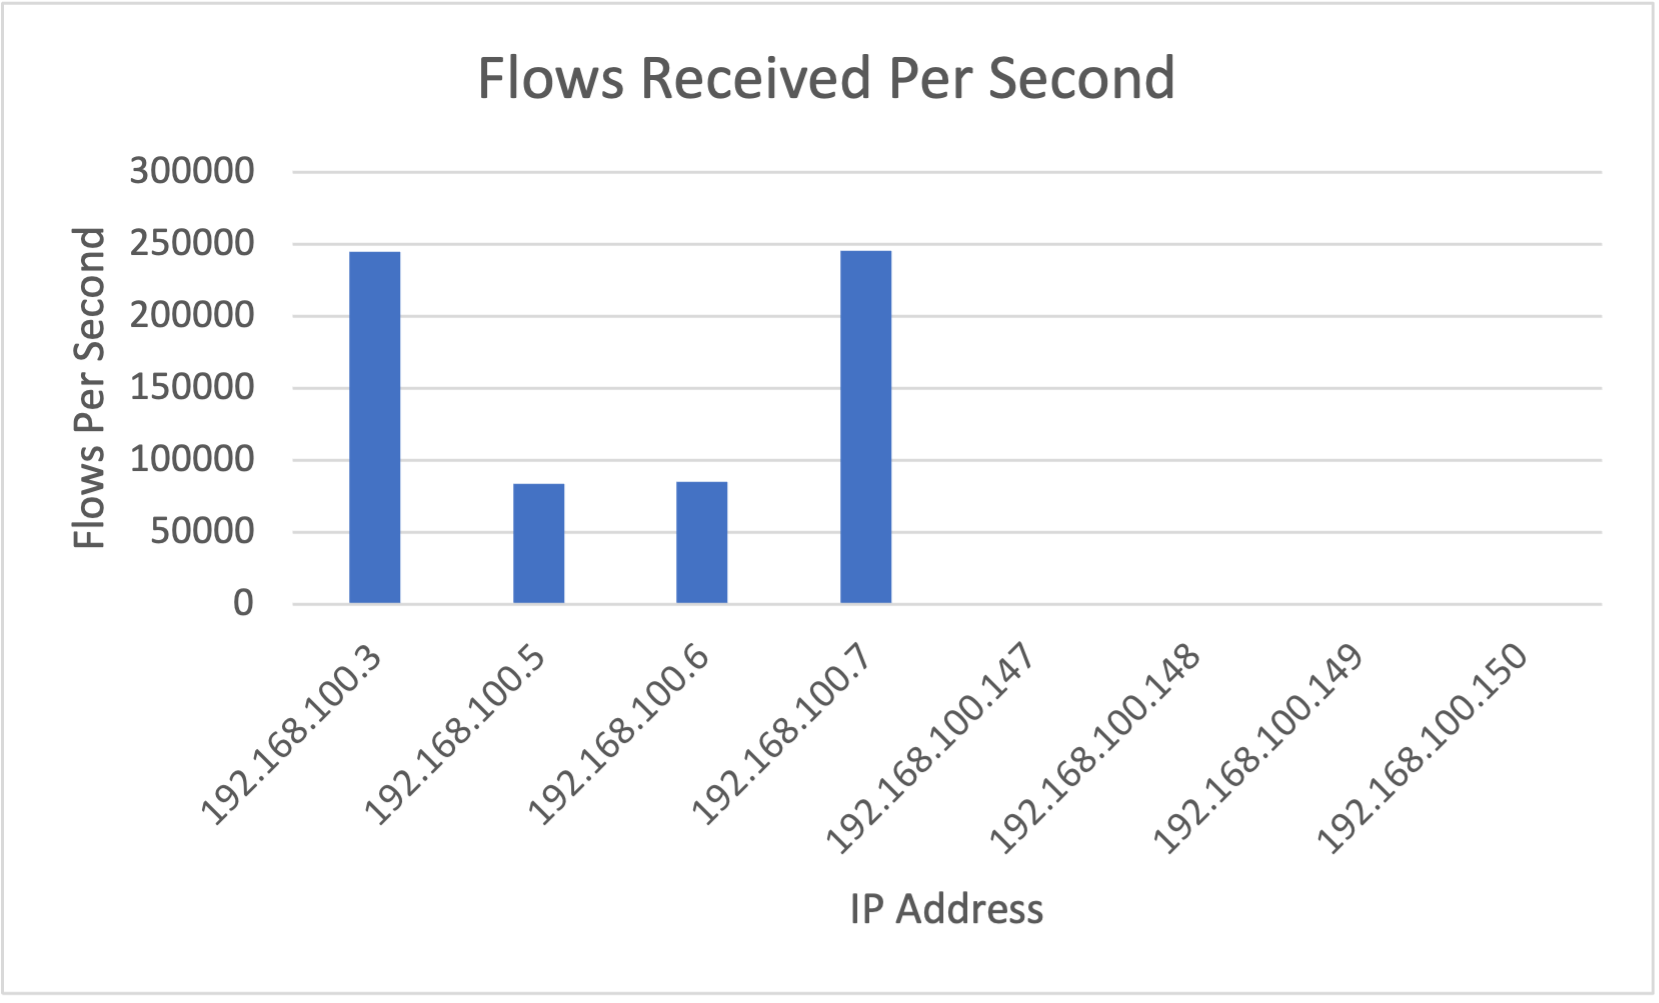
\includegraphics[width=8cm]{Figure4.png}
    \centering
    \caption{The number of flows that were sent to particular IP addresses per second}
    \label{fig:senttopersec}
\end{figure}

\begin{figure}[h]
    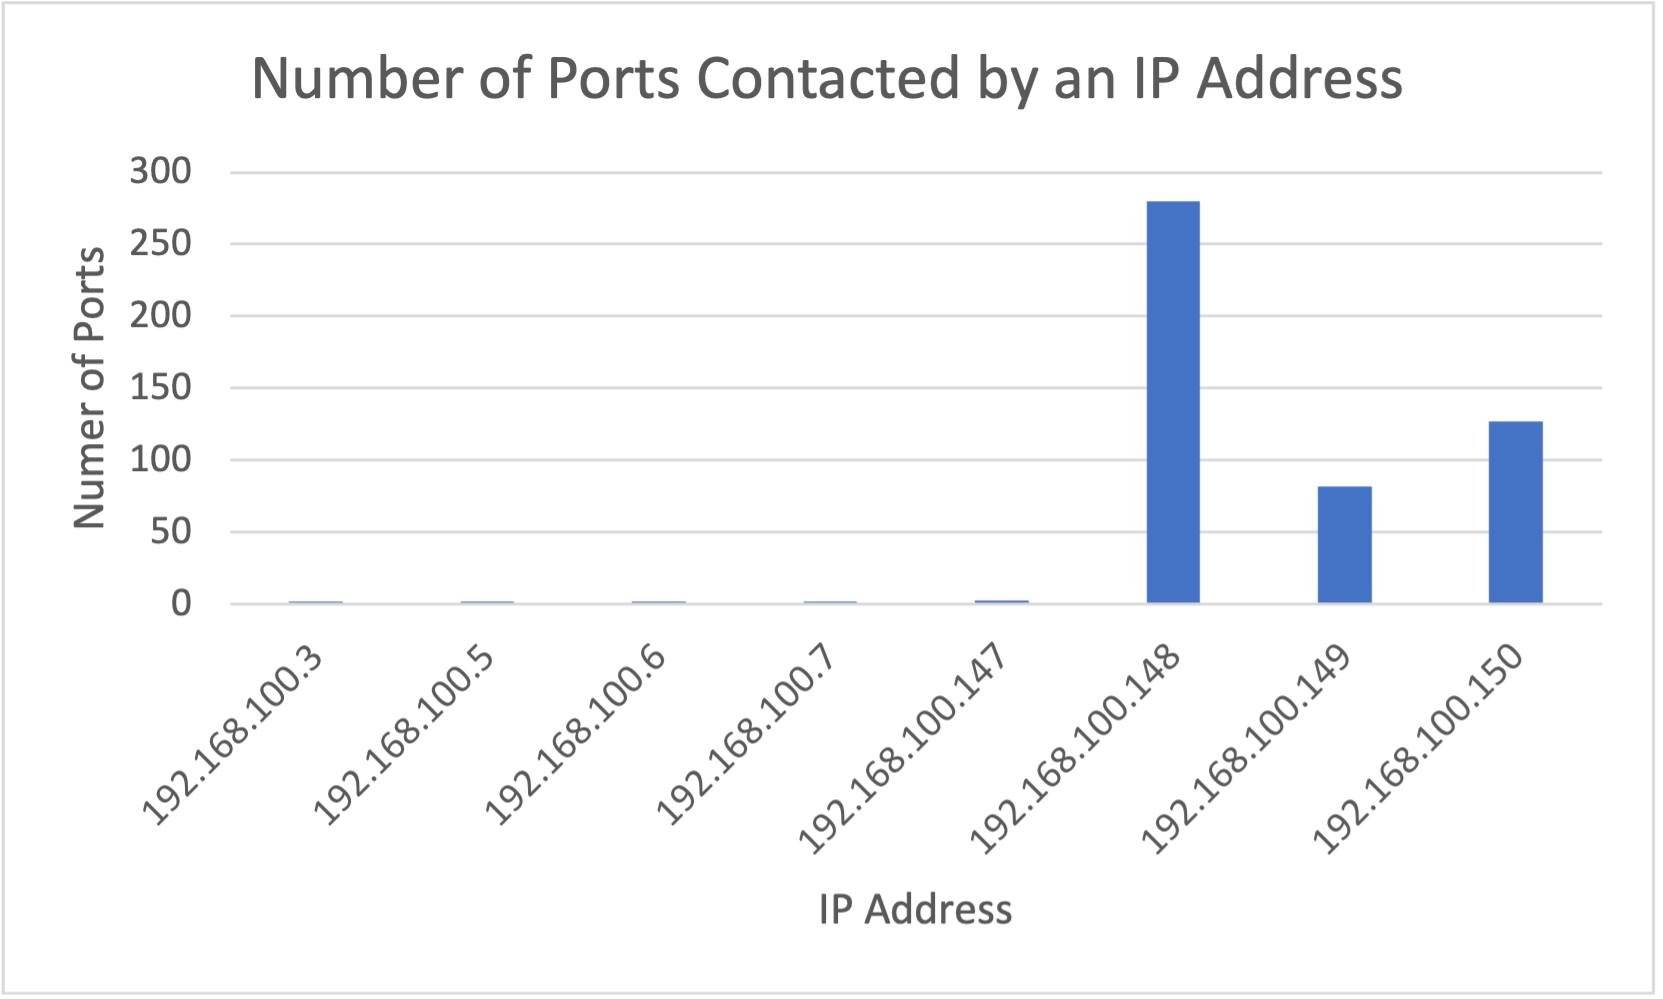
\includegraphics[width=8cm]{Figure5.png}
    \centering
    \caption{The number of ports contacted per IP address}
    \label{fig:portscontacted}
\end{figure}

\begin{figure}[h]
    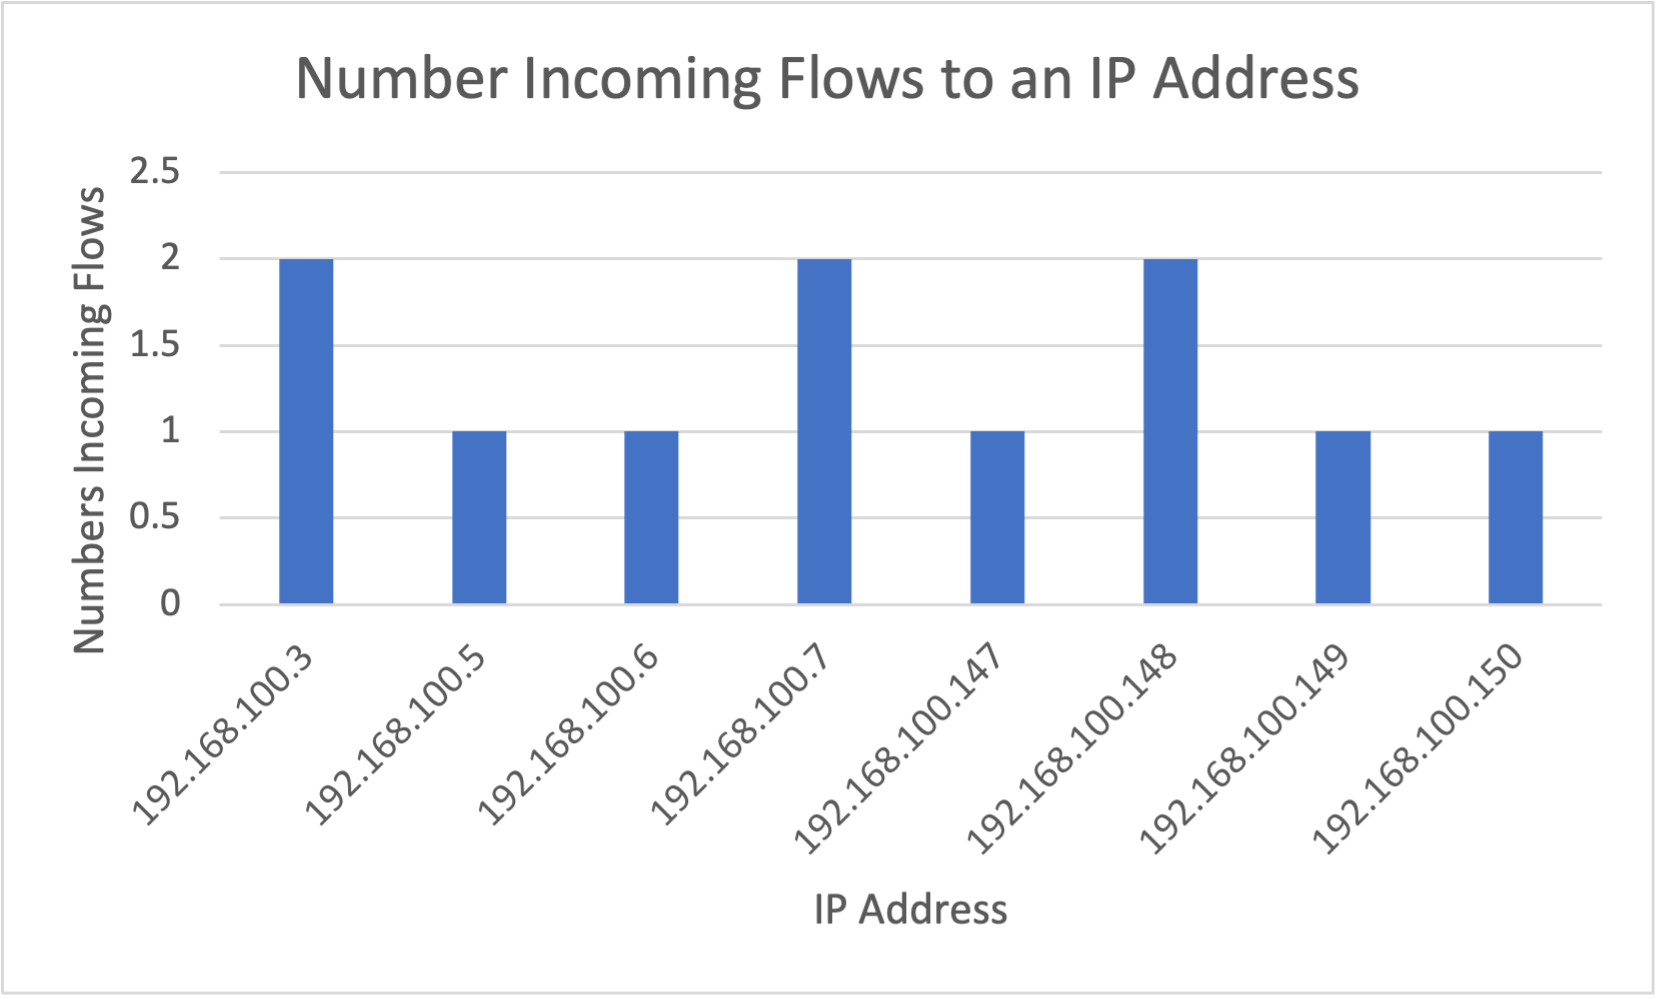
\includegraphics[width=8cm]{Figure6.png}
    \centering
    \caption{The number of flows from unique IP addresses coming into a particular IP address}
    \label{fig:incomingflows}
\end{figure}

\section{Analysis}

\section{Future Work}

\section{Conclusion}

\printbibliography

\end{document}